\chapter{Spanning trees}

\index{spanning tree}

A \key{spanning tree} is a set of edges of a graph
such that there is a path between any two nodes
in the graph using only the edges in the spanning tree.
Like trees in general, a spanning tree is
connected and acyclic.
Usually, there are many ways to construct a spanning tree.

For example, in the graph
\begin{center}
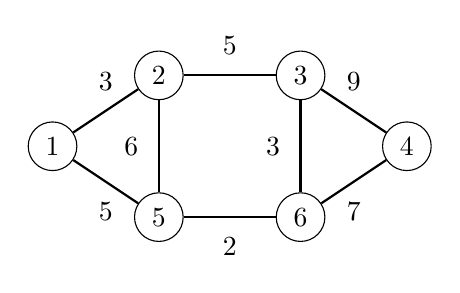
\begin{tikzpicture}[scale=0.9]
\node[draw, circle] (1) at (1.5,2) {$1$};
\node[draw, circle] (2) at (3,3) {$2$};
\node[draw, circle] (3) at (5,3) {$3$};
\node[draw, circle] (4) at (6.5,2) {$4$};
\node[draw, circle] (5) at (3,1) {$5$};
\node[draw, circle] (6) at (5,1) {$6$};
\path[draw,thick,-] (1) -- node[font=\small,label=above:3] {} (2);
\path[draw,thick,-] (2) -- node[font=\small,label=above:5] {} (3);
\path[draw,thick,-] (3) -- node[font=\small,label=above:9] {} (4);
\path[draw,thick,-] (1) -- node[font=\small,label=below:5] {} (5);
\path[draw,thick,-] (5) -- node[font=\small,label=below:2] {} (6);
\path[draw,thick,-] (6) -- node[font=\small,label=below:7] {} (4);
\path[draw,thick,-] (2) -- node[font=\small,label=left:6] {} (5);
\path[draw,thick,-] (3) -- node[font=\small,label=left:3] {} (6);
\end{tikzpicture}
\end{center}
one possible spanning tree is as follows:
\begin{center}
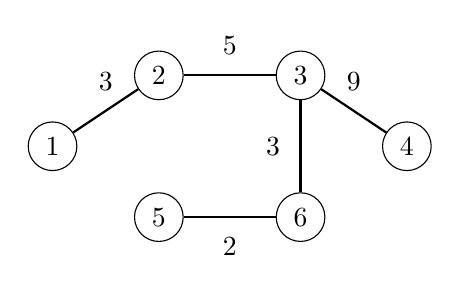
\begin{tikzpicture}[scale=0.9]
\node[draw, circle] (1) at (1.5,2) {$1$};
\node[draw, circle] (2) at (3,3) {$2$};
\node[draw, circle] (3) at (5,3) {$3$};
\node[draw, circle] (4) at (6.5,2) {$4$};
\node[draw, circle] (5) at (3,1) {$5$};
\node[draw, circle] (6) at (5,1) {$6$};
\path[draw,thick,-] (1) -- node[font=\small,label=above:3] {} (2);
\path[draw,thick,-] (2) -- node[font=\small,label=above:5] {} (3);
\path[draw,thick,-] (3) -- node[font=\small,label=above:9] {} (4);
\path[draw,thick,-] (5) -- node[font=\small,label=below:2] {} (6);
\path[draw,thick,-] (3) -- node[font=\small,label=left:3] {} (6);
\end{tikzpicture}
\end{center}

The weight of a spanning tree is the sum of the edge weights.
For example, the weight of the above spanning tree is
$3+5+9+3+2=22$.

\index{minimum spanning tree}

A \key{minimum spanning tree}
is a spanning tree whose weight is as small as possible.
The weight of a minimum spanning tree for the above graph
is 20, and a tree can be constructed as follows:

\begin{center}
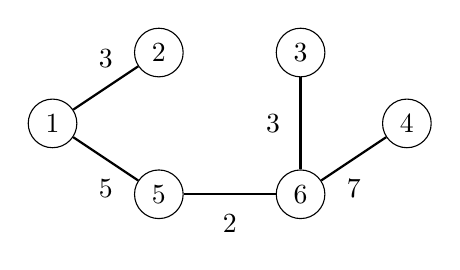
\begin{tikzpicture}[scale=0.9]
\node[draw, circle] (1) at (1.5,2) {$1$};
\node[draw, circle] (2) at (3,3) {$2$};
\node[draw, circle] (3) at (5,3) {$3$};
\node[draw, circle] (4) at (6.5,2) {$4$};
\node[draw, circle] (5) at (3,1) {$5$};
\node[draw, circle] (6) at (5,1) {$6$};

\path[draw,thick,-] (1) -- node[font=\small,label=above:3] {} (2);
%\path[draw,thick,-] (2) -- node[font=\small,label=above:5] {} (3);
%\path[draw,thick,-] (3) -- node[font=\small,label=above:9] {} (4);
\path[draw,thick,-] (1) -- node[font=\small,label=below:5] {} (5);
\path[draw,thick,-] (5) -- node[font=\small,label=below:2] {} (6);
\path[draw,thick,-] (6) -- node[font=\small,label=below:7] {} (4);
%\path[draw,thick,-] (2) -- node[font=\small,label=left:6] {} (5);
\path[draw,thick,-] (3) -- node[font=\small,label=left:3] {} (6);
\end{tikzpicture}
\end{center}

\index{maximum spanning tree}

Correspondingly, a \key{maximum spanning tree}
is a spanning tree whose weight is as large as possible.
The weight of a maximum spanning tree for the
above graph is 32:

\begin{center}
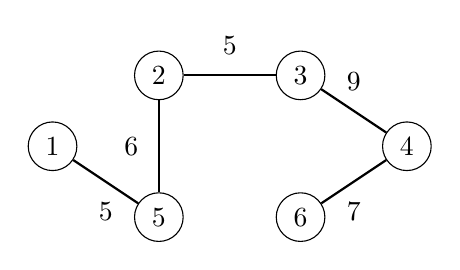
\begin{tikzpicture}[scale=0.9]
\node[draw, circle] (1) at (1.5,2) {$1$};
\node[draw, circle] (2) at (3,3) {$2$};
\node[draw, circle] (3) at (5,3) {$3$};
\node[draw, circle] (4) at (6.5,2) {$4$};
\node[draw, circle] (5) at (3,1) {$5$};
\node[draw, circle] (6) at (5,1) {$6$};
%\path[draw,thick,-] (1) -- node[font=\small,label=above:3] {} (2);
\path[draw,thick,-] (2) -- node[font=\small,label=above:5] {} (3);
\path[draw,thick,-] (3) -- node[font=\small,label=above:9] {} (4);
\path[draw,thick,-] (1) -- node[font=\small,label=below:5] {} (5);
%\path[draw,thick,-] (5) -- node[font=\small,label=below:2] {} (6);
\path[draw,thick,-] (6) -- node[font=\small,label=below:7] {} (4);
\path[draw,thick,-] (2) -- node[font=\small,label=left:6] {} (5);
%\path[draw,thick,-] (3) -- node[font=\small,label=left:3] {} (6);
\end{tikzpicture}
\end{center}

Note that there may be several different ways
for constructing a minimum or maximum spanning tree,
so the trees are not unique.

This chapter discusses algorithms that construct
a minimum or maximum spanning tree for a graph.
It turns out that it is easy to find such spanning trees
because many greedy methods produce an optimal solution.

We will learn two algorithms that both construct the
tree by choosing edges ordered by weights.
We will focus on finding a minimum spanning tree,
but the same algorithms can be used for finding a
maximum spanning tree by processing the edges in reverse order.

\section{Kruskal's algorithm}

\index{Kruskal's algorithm}

In \key{Kruskal's algorithm}, the initial spanning tree
is empty and doesn't contain any edges.
Then the algorithm adds edges to the tree
one at a time
in increasing order of their weights.
At each step, the algorithm includes an edge in the tree
if it doesn't create a cycle.

Kruskal's algorithm maintains the components
in the tree.
Initially, each node of the graph
is in its own component,
and each edge added to the tree joins two components.
Finally, all nodes will be in the same component,
and a minimum spanning tree has been found.

\subsubsection{Example}

\begin{samepage}
Let's consider how Kruskal's algorithm processes the
following graph:
\begin{center}
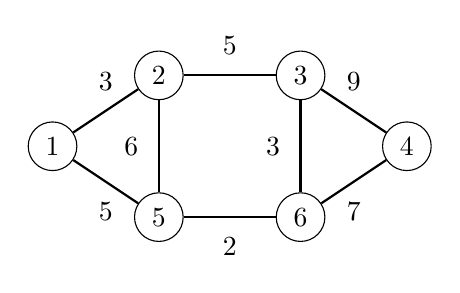
\begin{tikzpicture}[scale=0.9]
\node[draw, circle] (1) at (1.5,2) {$1$};
\node[draw, circle] (2) at (3,3) {$2$};
\node[draw, circle] (3) at (5,3) {$3$};
\node[draw, circle] (4) at (6.5,2) {$4$};
\node[draw, circle] (5) at (3,1) {$5$};
\node[draw, circle] (6) at (5,1) {$6$};
\path[draw,thick,-] (1) -- node[font=\small,label=above:3] {} (2);
\path[draw,thick,-] (2) -- node[font=\small,label=above:5] {} (3);
\path[draw,thick,-] (3) -- node[font=\small,label=above:9] {} (4);
\path[draw,thick,-] (1) -- node[font=\small,label=below:5] {} (5);
\path[draw,thick,-] (5) -- node[font=\small,label=below:2] {} (6);
\path[draw,thick,-] (6) -- node[font=\small,label=below:7] {} (4);
\path[draw,thick,-] (2) -- node[font=\small,label=left:6] {} (5);
\path[draw,thick,-] (3) -- node[font=\small,label=left:3] {} (6);
\end{tikzpicture}
\end{center}
\end{samepage}

\begin{samepage}
The first step in the algorithm is to sort the
edges in increasing order of their weights.
The result is the following list:

\begin{tabular}{ll}
\\
edge & weight \\
\hline
5--6 & 2 \\
1--2 & 3 \\
3--6 & 3 \\
1--5 & 5 \\
2--3 & 5 \\
2--5 & 6 \\
4--6 & 7 \\
3--4 & 9 \\
\\
\end{tabular}
\end{samepage}

After this, the algorithm goes through the list
and adds an edge to the tree if it joins
two separate components.

Initially, each node is in its own component:

\begin{center}
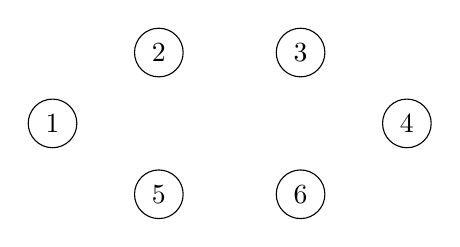
\begin{tikzpicture}[scale=0.9]
\node[draw, circle] (1) at (1.5,2) {$1$};
\node[draw, circle] (2) at (3,3) {$2$};
\node[draw, circle] (3) at (5,3) {$3$};
\node[draw, circle] (4) at (6.5,2) {$4$};
\node[draw, circle] (5) at (3,1) {$5$};
\node[draw, circle] (6) at (5,1) {$6$};
%\path[draw,thick,-] (1) -- node[font=\small,label=above:3] {} (2);
%\path[draw,thick,-] (2) -- node[font=\small,label=above:5] {} (3);
%\path[draw,thick,-] (3) -- node[font=\small,label=above:9] {} (4);
%\path[draw,thick,-] (1) -- node[font=\small,label=below:5] {} (5);
%\path[draw,thick,-] (5) -- node[font=\small,label=below:2] {} (6);
%\path[draw,thick,-] (6) -- node[font=\small,label=below:7] {} (4);
%\path[draw,thick,-] (2) -- node[font=\small,label=left:6] {} (5);
%\path[draw,thick,-] (3) -- node[font=\small,label=left:3] {} (6);
\end{tikzpicture}
\end{center}
The first edge to be added to the tree is
edge 5--6 that joins components
$\{5\}$ and $\{6\}$ into component $\{5,6\}$:

\begin{center}
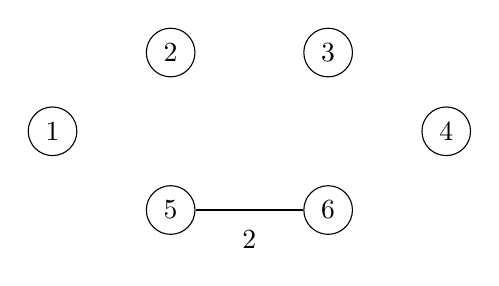
\begin{tikzpicture}
\node[draw, circle] (1) at (1.5,2) {$1$};
\node[draw, circle] (2) at (3,3) {$2$};
\node[draw, circle] (3) at (5,3) {$3$};
\node[draw, circle] (4) at (6.5,2) {$4$};
\node[draw, circle] (5) at (3,1) {$5$};
\node[draw, circle] (6) at (5,1) {$6$};

%\path[draw,thick,-] (1) -- node[font=\small,label=above:3] {} (2);
%\path[draw,thick,-] (2) -- node[font=\small,label=above:5] {} (3);
%\path[draw,thick,-] (3) -- node[font=\small,label=above:9] {} (4);
%\path[draw,thick,-] (1) -- node[font=\small,label=below:5] {} (5);
\path[draw,thick,-] (5) -- node[font=\small,label=below:2] {} (6);
%\path[draw,thick,-] (6) -- node[font=\small,label=below:7] {} (4);
%\path[draw,thick,-] (2) -- node[font=\small,label=left:6] {} (5);
%\path[draw,thick,-] (3) -- node[font=\small,label=left:3] {} (6);
\end{tikzpicture}
\end{center}
After this, edges 1--2, 3--6 and 1--5 are added in a similar way:

\begin{center}
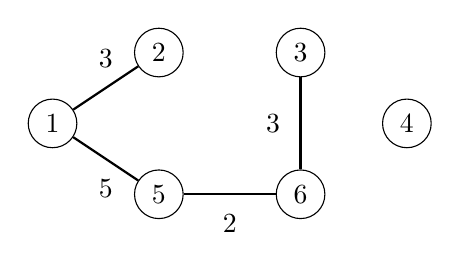
\begin{tikzpicture}[scale=0.9]
\node[draw, circle] (1) at (1.5,2) {$1$};
\node[draw, circle] (2) at (3,3) {$2$};
\node[draw, circle] (3) at (5,3) {$3$};
\node[draw, circle] (4) at (6.5,2) {$4$};
\node[draw, circle] (5) at (3,1) {$5$};
\node[draw, circle] (6) at (5,1) {$6$};

\path[draw,thick,-] (1) -- node[font=\small,label=above:3] {} (2);
%\path[draw,thick,-] (2) -- node[font=\small,label=above:5] {} (3);
%\path[draw,thick,-] (3) -- node[font=\small,label=above:9] {} (4);
\path[draw,thick,-] (1) -- node[font=\small,label=below:5] {} (5);
\path[draw,thick,-] (5) -- node[font=\small,label=below:2] {} (6);
%\path[draw,thick,-] (6) -- node[font=\small,label=below:7] {} (4);
%\path[draw,thick,-] (2) -- node[font=\small,label=left:6] {} (5);
\path[draw,thick,-] (3) -- node[font=\small,label=left:3] {} (6);
\end{tikzpicture}
\end{center}

After those steps, many components have been joined
and there are two components in the tree:
$\{1,2,3,5,6\}$ and $\{4\}$.

The next edge in the list is edge 2--3,
but it will not be included in the tree because
nodes 2 and 3 are already in the same component.
For the same reason, edge 2--5 will not be added
to the tree.

\begin{samepage}
Finally, edge 4--6 will be included in the tree:

\begin{center}
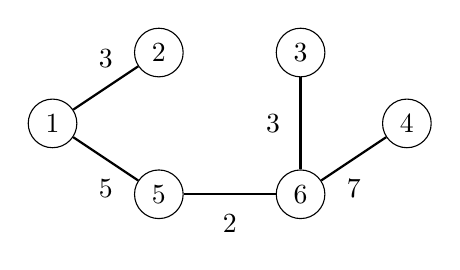
\begin{tikzpicture}[scale=0.9]
\node[draw, circle] (1) at (1.5,2) {$1$};
\node[draw, circle] (2) at (3,3) {$2$};
\node[draw, circle] (3) at (5,3) {$3$};
\node[draw, circle] (4) at (6.5,2) {$4$};
\node[draw, circle] (5) at (3,1) {$5$};
\node[draw, circle] (6) at (5,1) {$6$};

\path[draw,thick,-] (1) -- node[font=\small,label=above:3] {} (2);
%\path[draw,thick,-] (2) -- node[font=\small,label=above:5] {} (3);
%\path[draw,thick,-] (3) -- node[font=\small,label=above:9] {} (4);
\path[draw,thick,-] (1) -- node[font=\small,label=below:5] {} (5);
\path[draw,thick,-] (5) -- node[font=\small,label=below:2] {} (6);
\path[draw,thick,-] (6) -- node[font=\small,label=below:7] {} (4);
%\path[draw,thick,-] (2) -- node[font=\small,label=left:6] {} (5);
\path[draw,thick,-] (3) -- node[font=\small,label=left:3] {} (6);
\end{tikzpicture}
\end{center}
\end{samepage}

After this, the algorithm terminates because
there is a path between any two nodes and
the graph is connected.
The resulting graph is a minimum spanning tree
with weight $2+3+3+5+7=20$.

\subsubsection{Why does this work?}

It's a good question why Kruskal's algorithm works.
Why does the greedy strategy guarantee that we
will find a minimum spanning tree?

Let's see what happens if the lightest edge in
the graph is not included in the minimum spanning tree.
For example, assume that a minimum spanning tree
for the above graph would not contain the edge
between nodes 5 and 6 with weight 2.
We don't know exactly how the new minimum spanning tree
would look like, but still it has to contain some edges.
Assume that the tree would be as follows:

\begin{center}
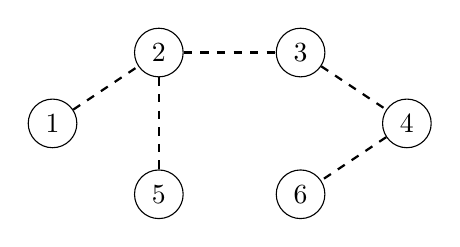
\begin{tikzpicture}[scale=0.9]
\node[draw, circle] (1) at (1.5,2) {$1$};
\node[draw, circle] (2) at (3,3) {$2$};
\node[draw, circle] (3) at (5,3) {$3$};
\node[draw, circle] (4) at (6.5,2) {$4$};
\node[draw, circle] (5) at (3,1) {$5$};
\node[draw, circle] (6) at (5,1) {$6$};

\path[draw,thick,-,dashed] (1) -- (2);
\path[draw,thick,-,dashed] (2) -- (5);
\path[draw,thick,-,dashed] (2) -- (3);
\path[draw,thick,-,dashed] (3) -- (4);
\path[draw,thick,-,dashed] (4) -- (6);
\end{tikzpicture}
\end{center}

However, it's not possible that the above tree
would be a real minimum spanning tree for the graph.
The reason for this is that we can remove an edge
from it and replace it with the edge with weight 2.
This produces a spanning tree whose weight is
\emph{smaller}:

\begin{center}
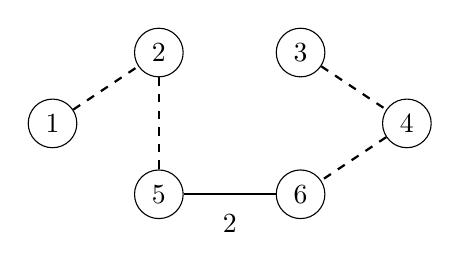
\begin{tikzpicture}[scale=0.9]
\node[draw, circle] (1) at (1.5,2) {$1$};
\node[draw, circle] (2) at (3,3) {$2$};
\node[draw, circle] (3) at (5,3) {$3$};
\node[draw, circle] (4) at (6.5,2) {$4$};
\node[draw, circle] (5) at (3,1) {$5$};
\node[draw, circle] (6) at (5,1) {$6$};

\path[draw,thick,-,dashed] (1) -- (2);
\path[draw,thick,-,dashed] (2) -- (5);
\path[draw,thick,-,dashed] (3) -- (4);
\path[draw,thick,-,dashed] (4) -- (6);
\path[draw,thick,-] (5) -- node[font=\small,label=below:2] {} (6);
\end{tikzpicture}
\end{center}

For this reason, it is always optimal to include the lightest edge
in the minimum spanning tree.
Using a similar argument, we can show that we
can also add the second lightest edge to the tree, and so on.
Thus, Kruskal's algorithm works correctly and
always produces a minimum spanning tree.

\subsubsection{Implementation}

Kruskal's algorithm can be conveniently
implemented using an edge list.
The first phase of the algorithm sorts the
edges in $O(m \log m)$ time.
After this, the second phase of the algorithm
builds the minimum spanning tree. 

The second phase of the algorithm looks as follows:

\begin{lstlisting}
for (...) {
  if (!same(a,b)) union(a,b);
}
\end{lstlisting}

The loop goes through the edges in the list
and always processes an edge $a$--$b$
where $a$ and $b$ are two nodes.
The code uses two functions:
the function \texttt{same} determines
if the nodes are in the same component,
and the function \texttt{unite}
joins two components into a single component.

The problem is how to efficiently implement
the functions \texttt{same} and \texttt{unite}.
One possibility is to maintain the graph
in a usual way and implement the function
\texttt{same} as graph traversal.
However, using this technique,
the running time of the function \texttt{same} would be $O(n+m)$,
and this would be slow because the function will be
called for each edge in the graph.

We will solve the problem using a union-find structure
that implements both the functions in $O(\log n)$ time.
Thus, the time complexity of Kruskal's algorithm
will be $O(m \log n)$ after sorting the edge list.

\section{Union-find structure}

\index{union-find structure}

The \key{union-find structure} maintains
a collection of sets.
The sets are disjoint, so no element
belongs to more than one set.
Two $O(\log n)$ time operations are supported.
The first operation checks if two elements
belong to the same set,
and the second operation joins two sets into a single set.

\subsubsection{Structure}

In the union-find structure, one element in each set
is the representative of the set.
All other elements in the set point to the
representative directly or through other elements in the set.
For example, in the following picture there are three sets:
$\{1,4,7\}$, $\{5\}$ and $\{2,3,6,8\}$.
\begin{center}
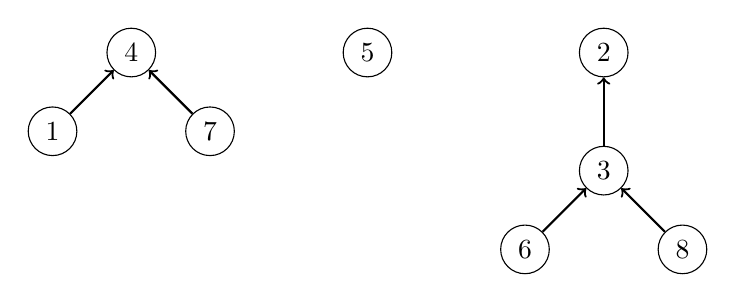
\begin{tikzpicture}
\node[draw, circle] (1) at (0,-1) {$1$};
\node[draw, circle] (2) at (7,0) {$2$};
\node[draw, circle] (3) at (7,-1.5) {$3$};
\node[draw, circle] (4) at (1,0) {$4$};
\node[draw, circle] (5) at (4,0) {$5$};
\node[draw, circle] (6) at (6,-2.5) {$6$};
\node[draw, circle] (7) at (2,-1) {$7$};
\node[draw, circle] (8) at (8,-2.5) {$8$};

\path[draw,thick,->] (1) -- (4);
\path[draw,thick,->] (7) -- (4);

\path[draw,thick,->] (3) -- (2);
\path[draw,thick,->] (6) -- (3);
\path[draw,thick,->] (8) -- (3);

\end{tikzpicture}
\end{center}
In this case the representatives
of the sets are 4, 5 and 2.
For each element, we can find the representative
for the corresponding set by following the
path that begins at the element.
For example, element 2 is the representative for the set
that contains element 6 because
the path is $6 \rightarrow 3 \rightarrow 2$.
Thus, two elements belong to the same set exactly when
they point to the same representative.

Two sets can be combined by connecting the
representative of one set to the
representative of another set.
For example, sets
$\{1,4,7\}$ and $\{2,3,6,8\}$
can be combined as follows into set $\{1,2,3,4,6,7,8\}$:
\begin{center}
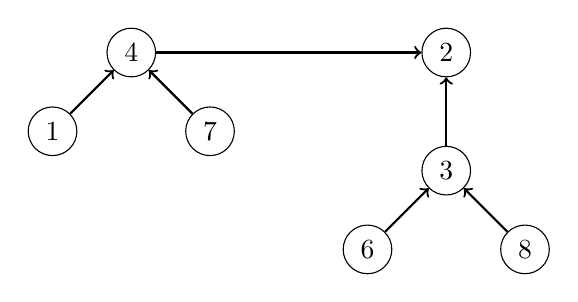
\begin{tikzpicture}
\node[draw, circle] (1) at (2,-1) {$1$};
\node[draw, circle] (2) at (7,0) {$2$};
\node[draw, circle] (3) at (7,-1.5) {$3$};
\node[draw, circle] (4) at (3,0) {$4$};
\node[draw, circle] (6) at (6,-2.5) {$6$};
\node[draw, circle] (7) at (4,-1) {$7$};
\node[draw, circle] (8) at (8,-2.5) {$8$};

\path[draw,thick,->] (1) -- (4);
\path[draw,thick,->] (7) -- (4);

\path[draw,thick,->] (3) -- (2);
\path[draw,thick,->] (6) -- (3);
\path[draw,thick,->] (8) -- (3);

\path[draw,thick,->] (4) -- (2);
\end{tikzpicture}
\end{center}

In this case, element 2 becomes the representative
for the whole set and the old representative 4
points to it.

The efficiency of the operations depends on
the way the sets are combined.
It turns out that we can follow a simple strategy
and always connect the representative of the
smaller set to the representative of the larger set
(or, if the sets are of the same size,
both choices are fine).
Using this strategy, the length of a path from
a element in a set to a representative is
always $O(\log n)$ because each step forward
in the path doubles the size of the corresponding set.

\subsubsection{Implementation}

We can implement the union-find structure
using arrays.
In the following implementation,
array \texttt{k} contains for each element
the next element
in the path, or the element itself if it is
a representative,
and array \texttt{s} indicates for each representative
the size of the corresponding set.

Initially, each element has an own set with size 1:
\begin{lstlisting}
for (int i = 1; i <= n; i++) k[i] = i;
for (int i = 1; i <= n; i++) s[i] = 1;
\end{lstlisting}

The function \texttt{find} returns
the representative for element $x$.
The representative can be found by following
the path that begins at element $x$.

\begin{lstlisting}
int find(int x) {
    while (x != k[x]) x = k[x];
    return x;
}
\end{lstlisting}

The function \texttt{same} finds out
whether elements $a$ and $b$ belong to the same set.
This can easily be done by using the
function \texttt{find}.

\begin{lstlisting}
bool same(int a, int b) {
    return find(a) == find(b);
}
\end{lstlisting}

\begin{samepage}
The function \texttt{union} combines the sets
that contain elements $a$ and $b$
into a single set.
The function first finds the representatives
of the sets and then connects the smaller
set to the larger set.

\begin{lstlisting}
void union(int a, int b) {
    a = find(a);
    b = find(b);
    if (s[b] > s[a]) swap(a,b);
    s[a] += s[b];
    k[b] = a;
}
\end{lstlisting}
\end{samepage}

The time complexity of the function \texttt{find}
is $O(\log n)$ assuming that the length of the
path is $O(\log n)$.
Thus, the functions \texttt{same} and \texttt{union}
also work in $O(\log n)$ time.
The function \texttt{union} ensures that the
length of each path is $O(\log n)$ by connecting
the smaller set to the larger set.

\section{Primin algoritmi}

\index{Primin algoritmi@Primin algoritmi}

\key{Primin algoritmi} on vaihtoehtoinen menetelmä
verkon pienimmän virittävän puun muodostamiseen.
Algoritmi aloittaa puun muodostamisen jostakin
verkon solmusta ja lisää puuhun aina kaaren,
joka on mahdollisimman kevyt ja joka
liittää puuhun uuden solmun.
Lopulta kaikki solmut on lisätty puuhun
ja pienin virittävä puu on valmis.

Primin algoritmin toiminta on lähellä
Dijkstran algoritmia.
Erona on, että Dijkstran algoritmissa valitaan
kaari, jonka kautta syntyy lyhin polku alkusolmusta
uuteen solmuun, mutta Primin algoritmissa
valitaan vain kevein kaari, joka johtaa uuteen solmuun.

\subsubsection{Esimerkki}

Tarkastellaan Primin algoritmin toimintaa
seuraavassa verkossa:

\begin{center}
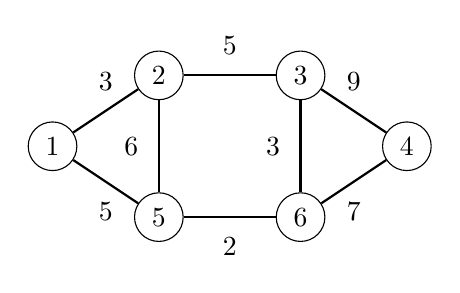
\begin{tikzpicture}[scale=0.9]
\node[draw, circle] (1) at (1.5,2) {$1$};
\node[draw, circle] (2) at (3,3) {$2$};
\node[draw, circle] (3) at (5,3) {$3$};
\node[draw, circle] (4) at (6.5,2) {$4$};
\node[draw, circle] (5) at (3,1) {$5$};
\node[draw, circle] (6) at (5,1) {$6$};
\path[draw,thick,-] (1) -- node[font=\small,label=above:3] {} (2);
\path[draw,thick,-] (2) -- node[font=\small,label=above:5] {} (3);
\path[draw,thick,-] (3) -- node[font=\small,label=above:9] {} (4);
\path[draw,thick,-] (1) -- node[font=\small,label=below:5] {} (5);
\path[draw,thick,-] (5) -- node[font=\small,label=below:2] {} (6);
\path[draw,thick,-] (6) -- node[font=\small,label=below:7] {} (4);
\path[draw,thick,-] (2) -- node[font=\small,label=left:6] {} (5);
\path[draw,thick,-] (3) -- node[font=\small,label=left:3] {} (6);

%\path[draw=red,thick,-,line width=2pt] (5) -- (6);
\end{tikzpicture}
\end{center}

Aluksi solmujen välillä ei ole mitään kaaria:
\begin{center}
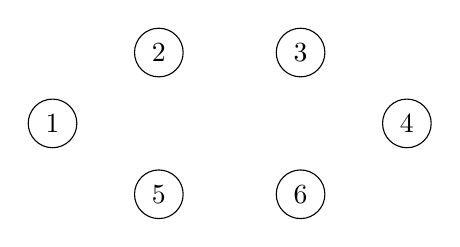
\begin{tikzpicture}[scale=0.9]
\node[draw, circle] (1) at (1.5,2) {$1$};
\node[draw, circle] (2) at (3,3) {$2$};
\node[draw, circle] (3) at (5,3) {$3$};
\node[draw, circle] (4) at (6.5,2) {$4$};
\node[draw, circle] (5) at (3,1) {$5$};
\node[draw, circle] (6) at (5,1) {$6$};
%\path[draw,thick,-] (1) -- node[font=\small,label=above:3] {} (2);
%\path[draw,thick,-] (2) -- node[font=\small,label=above:5] {} (3);
%\path[draw,thick,-] (3) -- node[font=\small,label=above:9] {} (4);
%\path[draw,thick,-] (1) -- node[font=\small,label=below:5] {} (5);
%\path[draw,thick,-] (5) -- node[font=\small,label=below:2] {} (6);
%\path[draw,thick,-] (6) -- node[font=\small,label=below:7] {} (4);
%\path[draw,thick,-] (2) -- node[font=\small,label=left:6] {} (5);
%\path[draw,thick,-] (3) -- node[font=\small,label=left:3] {} (6);
\end{tikzpicture}
\end{center}

Puun muodostuksen voi aloittaa mistä tahansa solmusta,
ja aloitetaan se nyt solmusta 1.
Kevein kaari on painoltaan 3 ja se johtaa solmuun 2:
\begin{center}
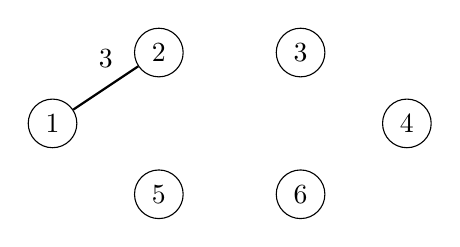
\begin{tikzpicture}[scale=0.9]
\node[draw, circle] (1) at (1.5,2) {$1$};
\node[draw, circle] (2) at (3,3) {$2$};
\node[draw, circle] (3) at (5,3) {$3$};
\node[draw, circle] (4) at (6.5,2) {$4$};
\node[draw, circle] (5) at (3,1) {$5$};
\node[draw, circle] (6) at (5,1) {$6$};
\path[draw,thick,-] (1) -- node[font=\small,label=above:3] {} (2);
%\path[draw,thick,-] (2) -- node[font=\small,label=above:5] {} (3);
%\path[draw,thick,-] (3) -- node[font=\small,label=above:9] {} (4);
%\path[draw,thick,-] (1) -- node[font=\small,label=below:5] {} (5);
%\path[draw,thick,-] (5) -- node[font=\small,label=below:2] {} (6);
%\path[draw,thick,-] (6) -- node[font=\small,label=below:7] {} (4);
%\path[draw,thick,-] (2) -- node[font=\small,label=left:6] {} (5);
%\path[draw,thick,-] (3) -- node[font=\small,label=left:3] {} (6);
\end{tikzpicture}
\end{center}

Nyt kevein uuteen solmuun johtavan
kaaren paino on 5,
ja voimme laajentaa joko solmuun 3 tai 5.
Valitaan solmu 3:
\begin{center}
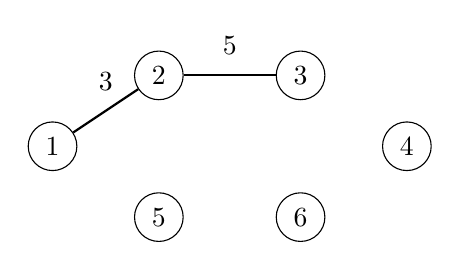
\begin{tikzpicture}[scale=0.9]
\node[draw, circle] (1) at (1.5,2) {$1$};
\node[draw, circle] (2) at (3,3) {$2$};
\node[draw, circle] (3) at (5,3) {$3$};
\node[draw, circle] (4) at (6.5,2) {$4$};
\node[draw, circle] (5) at (3,1) {$5$};
\node[draw, circle] (6) at (5,1) {$6$};
\path[draw,thick,-] (1) -- node[font=\small,label=above:3] {} (2);
\path[draw,thick,-] (2) -- node[font=\small,label=above:5] {} (3);
%\path[draw,thick,-] (3) -- node[font=\small,label=above:9] {} (4);
%\path[draw,thick,-] (1) -- node[font=\small,label=below:5] {} (5);
%\path[draw,thick,-] (5) -- node[font=\small,label=below:2] {} (6);
%\path[draw,thick,-] (6) -- node[font=\small,label=below:7] {} (4);
%\path[draw,thick,-] (2) -- node[font=\small,label=left:6] {} (5);
%\path[draw,thick,-] (3) -- node[font=\small,label=left:3] {} (6);
\end{tikzpicture}
\end{center}

\begin{samepage}
Sama jatkuu, kunnes kaikki solmut ovat mukana puussa:
\begin{center}
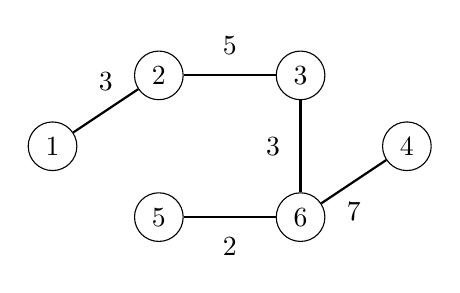
\begin{tikzpicture}[scale=0.9]
\node[draw, circle] (1) at (1.5,2) {$1$};
\node[draw, circle] (2) at (3,3) {$2$};
\node[draw, circle] (3) at (5,3) {$3$};
\node[draw, circle] (4) at (6.5,2) {$4$};
\node[draw, circle] (5) at (3,1) {$5$};
\node[draw, circle] (6) at (5,1) {$6$};
\path[draw,thick,-] (1) -- node[font=\small,label=above:3] {} (2);
\path[draw,thick,-] (2) -- node[font=\small,label=above:5] {} (3);
%\path[draw,thick,-] (3) -- node[font=\small,label=above:9] {} (4);
%\path[draw,thick,-] (1) -- node[font=\small,label=below:5] {} (5);
\path[draw,thick,-] (5) -- node[font=\small,label=below:2] {} (6);
\path[draw,thick,-] (6) -- node[font=\small,label=below:7] {} (4);
%\path[draw,thick,-] (2) -- node[font=\small,label=left:6] {} (5);
\path[draw,thick,-] (3) -- node[font=\small,label=left:3] {} (6);
\end{tikzpicture}
\end{center}
\end{samepage}

\subsubsection{Toteutus}

Dijkstran algoritmin tavoin Primin algoritmin voi toteuttaa
tehokkaasti käyttämällä prioriteettijonoa.
Primin algoritmin tapauksessa jono sisältää kaikki solmut,
jotka voi yhdistää nykyiseen komponentiin kaarella,
järjestyksessä kaaren painon mukaan kevyimmästä raskaimpaan.

Primin algoritmin aikavaativuus on $O(n + m \log m)$
eli sama kuin Dijkstran algoritmissa.
Käytännössä Primin algoritmi on suunnilleen
yhtä nopea kuin Kruskalin algoritmi,
ja onkin makuasia, kumpaa algoritmia käyttää.
Useimmat kisakoodarit käyttävät kuitenkin Kruskalin algoritmia.


